\chapter{Peruuttava haku}

\index{backtracking}
\emph{Peruuttava haku} (\emph{backtracking}) on menetelmä,
jossa on ideana käydä läpi kaikki mahdolliset tavat 
ratkaista annettu tehtävä.
Peruuttava haku on luontevaa toteuttaa rekursion avulla,
jolloin jokainen rekursion haara vastaa yhtä tapaa
viedä ratkaisua eteenpäin.

Tässä luvussa tutustumme ensin peruuttavan haun algoritmeihin,
jotka käyvät läpi lukujen yhdistelmiä.
Tämän jälkeen näemme, miten peruuttavaa hakua voi käyttää
kahdessa vaikeammassa ongelmassa ja miten hakua voi optimoida.
Lopuksi toteutamme pelin tekoälyn minmax-algoritmilla,
joka perustuu peruuttavaan hakuun.

\section{Silmukoista rekursioon}

Ensimmäinen tehtävämme on muodostaa kaikki yhdistelmät,
joissa on peräk\-käin $n$ kokonaislukua väliltä $1 \dots m$.
Tällaisia yhdistelmiä on kaikkiaan $m^n$,
koska joka kohdassa on $m$ tapaa valita kyseiseen kohtaan tuleva luku.
Esimerkiksi jos $n=3$ ja $m=4$, mahdollisia yhdistelmiä
ovat esimerkiksi $[1,2,1]$ ja $[3,1,4]$
ja yhdistelmiä on yhteensä $4^3=64$.

Luonteva tapa ratkaista tehtävä tietylle $n$:n arvolle on
luoda $n$ sisäkkäistä silmukkaa, joista jokainen käy $m$ lukua läpi.
Esimerkiksi seuraava koodi käy läpi kaikki yhdistelmät
tapauksessa $n=3$ ja $m=4$:

\begin{code}
for a = 1 to m
    for b = 1 to m
        for c = 1 to m
            print(a,b,c)
\end{code}

Tämä on sinänsä mainio ratkaisu, mutta siinä on yksi ongelma:
lukujen määrä $n$ vaikuttaa silmukoiden määrään.
Jos haluaisimme muuttaa $n$:n arvoa, meidän täytyisi muuttaa
koodin silmukoiden määrää, mikä ei ole hyvä asia.
Peruuttavan haun avulla voimme kuitenkin toteuttaa ratkaisun
rekursiivisesti niin, että sama koodi toimii kaikille $n$:n arvoille.

\subsection{Haun toteuttaminen}

Seuraava rekursiivinen proseduuri \texttt{haku} muodostaa
yhdistelmiä peruuttavan haun avulla.
Parametri $k$ tarkoittaa kohtaa, johon seuraava luku asetetaan.
Jos $k=n$, jokin yhdistelmä on valmistunut, jolloin se tulostetaan.
Muuten haku käy läpi kaikki tavat sijoittaa kohtaan $k$ luku $1 \dots m$
ja jatkaa rekursiivisesti kohtaan $k+1$.
Haku lähtee käyntiin kutsulla \texttt{haku}(0),
ja \texttt{luvut} on $n$-kokoinen taulukko, johon yhdistelmä muodostetaan.

\begin{code}
procedure haku(k)
    if k == n
        print(luvut)
    else
        for i = 1 to m
            luvut[k] = i
            haku(k+1)
\end{code}

Kuva \ref{fig:perhak} näyttää, miten peruuttava haku lähtee liikkeelle
tapauksessa $n=3$ ja $m=4$.
Merkki "$-$" tarkoittaa lukua, jota ei ole vielä valittu.
Haun ensimmäinen taso valitsee yhdistelmän
ensimmäisen luvun kohtaan $0$.
Tämän valintaan on neljä vaihtoehtoa ($1 \dots 4$),
joten haku haarautuu neljään osaan valitsemaan lukua kohtaan $1$.
Jokainen haara jatkaa vastaavasti eteenpäin
ja valitsee muut yhdistelmään kuuluvat luvut.

\begin{figure}
\center
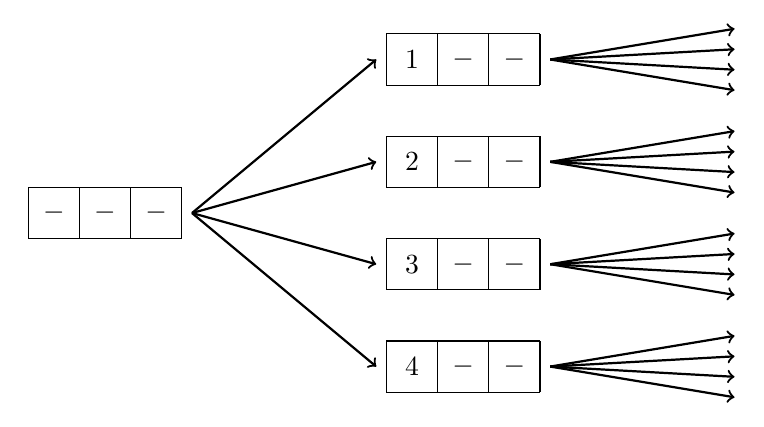
\begin{tikzpicture}[scale=.65]
    \draw (0,0) grid (3,1);
    \foreach \x/\v in {0/-,1/-,2/-} \node at (\x+0.5,0.5) {$\v$};

    \draw (7,-3) grid (10,-2);
    \foreach \x/\v in {0/1,1/-,2/-} \node at (\x+7.5,3.5) {$\v$};
    \draw (7,-1) grid (10,0);
    \foreach \x/\v in {0/2,1/-,2/-} \node at (\x+7.5,1.5) {$\v$};
    \draw (7,1) grid (10,2);
    \foreach \x/\v in {0/3,1/-,2/-} \node at (\x+7.5,-0.5) {$\v$};
    \draw (7,3) grid (10,4);
    \foreach \x/\v in {0/4,1/-,2/-} \node at (\x+7.5,-2.5) {$\v$};

    \draw[->,thick] (3.2,0.5) -- (6.8,3.5);
    \draw[->,thick] (3.2,0.5) -- (6.8,1.5);
    \draw[->,thick] (3.2,0.5) -- (6.8,-0.5);
    \draw[->,thick] (3.2,0.5) -- (6.8,-2.5);
    
    \foreach \y in {3.5,1.5,-0.5,-2.5} \foreach \z in {0.6,0.2,-0.2,-0.6}
        \draw[->,thick] (10.2,\y) -- (13.8,\y+\z);
\end{tikzpicture}
\caption{Peruuttavan haun alku tapauksessa $n=3$ ja $m=4$.}
\label{fig:perhak}
\end{figure}

Voimme arvioida algoritmin tehokkuutta laskemalla,
montako kertaa proseduuria \texttt{haku} kutsutaan yhteensä haun aikana.
Proseduuria kutsutaan kerran parametrilla $0$,
$m$ kertaa parametrilla $1$, $m^2$ kertaa parametrilla $2$, jne.,
joten kutsujen määrä on yhteensä
\[
1+m+m^2+\dots+m^n = \frac{m^{n+1}-1}{m-1} = O(m^n).
\]
Koska haku haarautuu joka tasolla $m$ osaan,
aikavaativuus kasvaa eksponentiaalisesti ja viimeisellä
tasolla tehdään enemmän kutsuja kuin kaikilla muilla tasoilla yhteensä.

\subsection{Osajoukot ja permutaatiot}

Tarkastellaan sitten ongelmaa,
jossa haluamme käydä läpi annetun joukon \emph{osajoukot}
eli kaikki tavat valita jokin osa joukon alkioista.
Esimerkiksi joukon $\{2,3,5,9\}$ osajoukkoja ovat
$\{2,5\}$ ja $\{3,5,9\}$.
Kun joukossa on $n$ alkiota, sillä on kaikkiaan $2^n$ osajoukkoa.

Osoittautuu, että voimme käydä läpi osajoukot lähes samalla
tavalla kuin aiemmassa ongelmassa.
Voimme näet muodostaa kaikki $n$-kokoiset yhdistelmät,
joissa jokainen luku on 0 tai 1.
Jokainen tällainen yhdistelmä vastaa yhtä osajoukkoa,
kun tulkintana on, että 1 valitsee alkion mukaan
ja 0 jättää sen pois.
Esimerkiksi joukon $\{2,3,5,9\}$ osajoukkoa $\{2,5\}$
vastaa yhdistelmä $[1,0,1,0]$,
koska luvut 2 ja 5 otetaan mukaan ja luvut 3 ja 9 jäävät pois.

Toinen tavallinen ongelma on muodostaa annetun joukon
\emph{permutaatiot} eli erilaiset järjestykset.
Esimerkiksi joukon $\{1,2,3,4\}$ permutaatioita ovat
$\{2,4,1,3\}$ ja $\{4,3,1,2\}$.
Kun joukossa on $n$ alkiota, siitä voidaan muodostaa
kaikkiaan $n!$ permutaatiota.

Tässäkin tapauksessa voimme ratkaista ongelman yhdistelmien
muodostamisen avulla.
Kun haluamme käydä läpi joukon $\{1,2,\dots,n\}$ permutaatiot,
muodostamme $n$-kokoisia yhdistelmiä, joissa jokainen luku
on väliltä $1 \dots n$.
Kuitenkin lisärajoituksena sama luku ei saa esiintyä monta kertaa,
joten kun olemme valinneet tietyn luvun,
emme voi enää valita sitä myöhemmin uudestaan.
Esimerkiksi jos $n=4$ ja permutaation alku on $[2,4,-,-]$,
voimme valita seuraavaan kohtaan vain luvun 1 tai 3.


\section{Esimerkki: Kuningatarongelma}

Klassinen tehtävä on selvittää,
monellako tavalla shakkilaudalle voidaan asettaa kahdeksan kuningatarta
niin, etteivät ne uhkaa toisiaan.
Käsittelemme seuraavaksi tämän tehtävän yleistystä,
jossa haluamme asettaa $n$ kuningatarta $n \times n$ -laudalle.
Esimerkiksi tapauksessa $n=4$ mahdollisia sijoitustapoja on 2,
jotka on esitetty kuvassa \ref{fig:kuning}.


\begin{figure}
\center
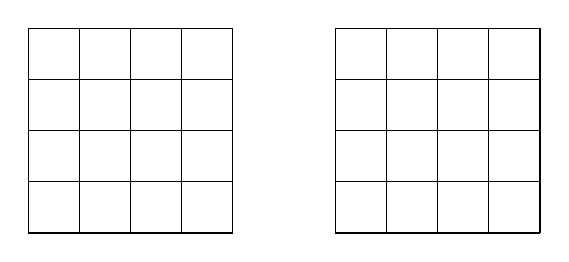
\begin{tikzpicture}[scale=.65]
  \begin{scope}
    \draw (0, 0) grid (4, 4);
    \node at (1.5,3.5) {$\symqueen$};
    \node at (3.5,2.5) {$\symqueen$};
    \node at (0.5,1.5) {$\symqueen$};
    \node at (2.5,0.5) {$\symqueen$};

    \draw (6, 0) grid (10, 4);
    \node at (6+2.5,3.5) {$\symqueen$};
    \node at (6+0.5,2.5) {$\symqueen$};
    \node at (6+3.5,1.5) {$\symqueen$};
    \node at (6+1.5,0.5) {$\symqueen$};
  \end{scope}
\end{tikzpicture}
\caption{Mahdolliset tavat asettaa 4 kuningatarta $4 \times 4$ -shakkilaudalle.}
\label{fig:kuning}
\end{figure}

\subsection{Haun toteuttaminen}

Voimme ratkaista tehtävän peruuttavalla haulla toteuttamalla algoritmin,
joka käy laudan läpi ylhäältä alaspäin ja asettaa yhden kuningattaren
jokaiselle riville.
Kuva \ref{fig:hakupuu} esittää haun toimintaa tapauksessa $n=4$.
Ensimmäisen rivin kuningatar voidaan asettaa mihin tahansa sarakkeeseen,
mutta seuraavilla riveillä aiemmat valinnat rajoittavat hakua.
Kuvassa näkyy toisen kuningattaren sijoittaminen,
kun ensimmäinen kuningatar on sarakkeessa 2.
Tällöin ainoa vaihtoehto on, että toinen kuningatar on sarakkeessa 4,
koska kaikissa muissa tapauksissa kuningattaret uhkaisivat toisiaan.


\begin{figure}
\center
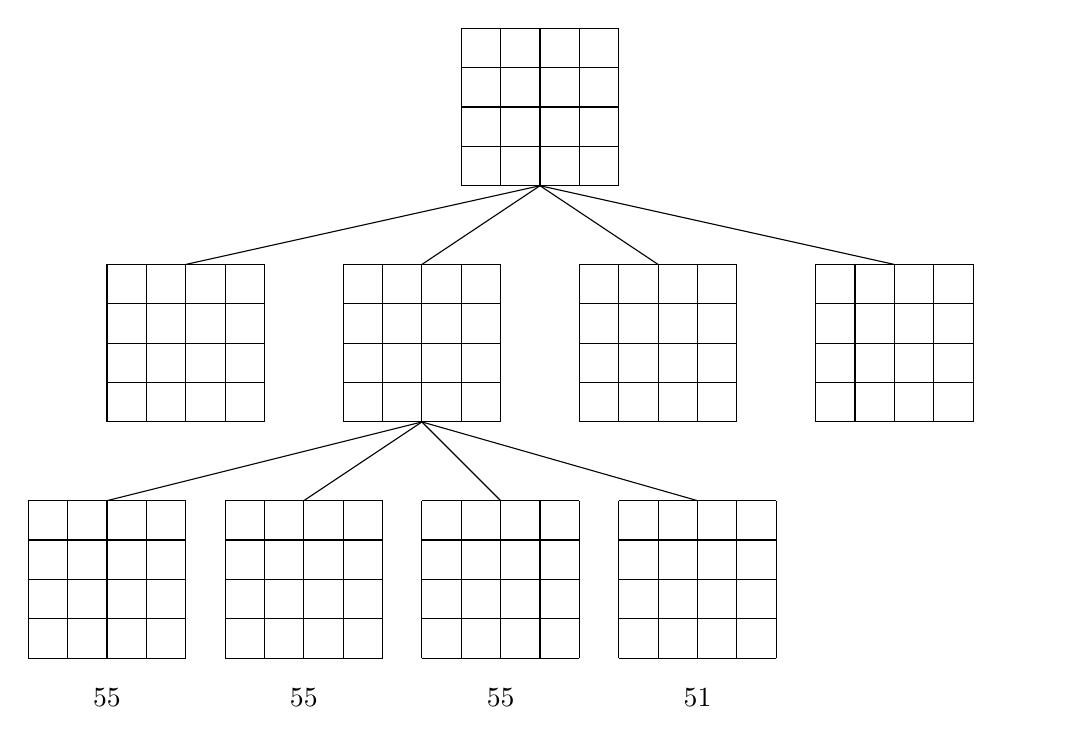
\begin{tikzpicture}[scale=.50]
  \begin{scope}
    \draw (0, 0) grid (4, 4);

    \draw (-9, -6) grid (-5, -2);
    \draw (-3, -6) grid (1, -2);
    \draw (3, -6) grid (7, -2);
    \draw (9, -6) grid (13, -2);

    \node at (-9+0.5,-3+0.5) {$\symqueen$};
    \node at (-3+1+0.5,-3+0.5) {$\symqueen$};
    \node at (3+2+0.5,-3+0.5) {$\symqueen$};
    \node at (9+3+0.5,-3+0.5) {$\symqueen$};

    \draw (2,0) -- (-7,-2);
    \draw (2,0) -- (-1,-2);
    \draw (2,0) -- (5,-2);
    \draw (2,0) -- (11,-2);

    \draw (-11, -12) grid (-7, -8);
    \draw (-6, -12) grid (-2, -8);
    \draw (-1, -12) grid (3, -8);
    \draw (4, -12) grid (8, -8);
    \draw[white] (11, -12) grid (15, -8);
    \node at (-11+1+0.5,-9+0.5) {$\symqueen$};
    \node at (-6+1+0.5,-9+0.5) {$\symqueen$};
    \node at (-1+1+0.5,-9+0.5) {$\symqueen$};
    \node at (4+1+0.5,-9+0.5) {$\symqueen$};
    \node at (-11+0+0.5,-10+0.5) {$\symqueen$};
    \node at (-6+1+0.5,-10+0.5) {$\symqueen$};
    \node at (-1+2+0.5,-10+0.5) {$\symqueen$};
    \node at (4+3+0.5,-10+0.5) {$\symqueen$};

    \draw (-1,-6) -- (-9,-8);
    \draw (-1,-6) -- (-4,-8);
    \draw (-1,-6) -- (1,-8);
    \draw (-1,-6) -- (6,-8);
    
    \node at (-9,-13) {\ding{55}};
    \node at (-4,-13) {\ding{55}};
    \node at (1,-13) {\ding{55}};
    \node at (6,-13) {\ding{51}};    
  \end{scope}
\end{tikzpicture}
\caption{Peruuttavan haun toiminta kuningatarongelmassa.}
\label{fig:hakupuu}
\end{figure}


Seuraava proseduuri \texttt{haku} esittää peruuttavan haun algoritmin,
joka etsii kuningatarongelman ratkaisut.
Oletamme, että laudan rivit ja sarakkeet on numeroitu $0,1,\dots,n-1$.
Parametri $y$ kertoo, mille riville seuraava kuningatar tulee sijoittaa,
ja haku lähtee käyntiin kutsulla \texttt{haku}$(0)$.
Jos rivinä on $n$, kaikki kuningattaret on jo sijoitettu,
joten yksi ratkaisu on löytynyt.
Muuten suoritetaan silmukka, joka käy läpi mahdolliset sarakkeet
muuttujan $x$ avulla.
Jos kuningatar voidaan sijoittaa sarakkeeseen $x$
eli se ei uhkaa mitään aiemmin sijoitettua kuningatarta,
merkitään taulukkoon \texttt{kohta},
että kuningatar $y$ on sarakkeessa $x$,
ja haku jatkuu eteenpäin rekursiivisesti.

\begin{code}
procedure haku(y)
    if y == n
        laskuri++
    else
        for x = 0 to n-1
            if voi_sijoittaa(y,x)
                kohta[y] = x
                haku(y+1)
\end{code}

Lisäksi täytyy toteuttaa funktio \texttt{voi\_sijoittaa},
joka tutkii, voidaanko uusi kuningatar sijoittaa
rivin $y$ sarakkeelle $x$.
Tämä voidaan selvittää taulukon \texttt{kohta} avulla näin:

\begin{code}
function voi_sijoittaa(y,x)
    for i = 0 to y-1
        if kohta[i] == x
            return false
        if abs(i-y) == abs(kohta[i]-x)
            return false
    return true
\end{code}

Funktio käy läpi kaikki aiemmin sijoitetut kuningattaret.
Jos aiemmin sijoitettu kuningatar olisi samassa sarakkeessa
(ensimmäinen ehto) tai samalla vinorivillä (toinen ehto)
kuin uusi kuningatar, tällaista sijoitusta ei voida tehdä
ja funktio palauttaa \texttt{false}.
Jos taas mikään aiempi kuningatar ei uhkaa uutta kuningatarta,
funktio palauttaa \texttt{true}.
Huomaa jälkimmäisessä ehdossa kätevä tapa tarkastaa,
ovatko kuningattaret samalla vinorivillä funktion \texttt{abs}
(itseisarvo) avulla.
Kuningattaret ovat samalla vinorivillä tarkalleen silloin,
kun niiden vaaka- ja pystysuuntaiset erot ovat samat.

Nyt meillä on valmis algoritmi, joiden avulla voimme etsiä
kuningatarongelman ratkaisuja.
Aina kun ratkaisu on valmis, taulukko \texttt{sarake} kertoo,
missä sarakkeissa kuningattaret ovat.
Esimerkiksi tapauksen $n=4$ ratkaisut (kuva \ref{fig:kuning})
vastaavat taulukoita $[1,3,0,2]$ ja $[2,0,3,1]$.
Voimme vaikkapa selvittää algoritmin avulla,
että tapauksessa $n=8$ eli tavallisella shakkilaudalla
ratkaisuja on yhteensä 92.

\subsection{Haun tehostaminen}

Peruuttavan haun algoritmit ovat usein hitaita,
koska ne joutuvat käymään läpi suuren määrän osittaisia ratkaisuja.
Voimme kuitenkin usein tehostaa hakua merkittävästi
toteuttamalla se paremmin.

Kuningatarongelmassa tapaus $n=8$ on vielä helppo ja
saamme laskettua tapojen määrän salamannopeasti,
mutta pian tämän jälkeen algoritmi alkaa hidastua tuntuvasti.
Tarkastelemme seuraavaksi tapausta $n=16$,
jossa sijoitustapojen määrä on 14772512.
Tässä tapauksessa yllä kuvatun algoritmin
Java-toteutus vie testikoneella aikaa 290 sekuntia.

\index{symmetria}
Yksi usein toimiva tapa tehostaa peruuttavan haun algoritmia
on ottaa huomioon \emph{symmetria}.
Kuningatarongelmassa hyödyllinen havainto on,
että jokaista ratkaisua vastaa toinen ratkaisu,
joka saadaan peilaamalla se vaakasuuntaisesti.
Niinpä voimme päättää, että asetamme ensimmäisen kuningattaren
laudan vasempaan osaan ($n/2$ ensimmäistä saraketta)
ja kerromme lopuksi vastauksen kahdella.
Tämä optimointi on hyvin helppo toteuttaa ja se puolittaa
laskenta-ajan: nyt algoritmi vie aikaa vain 145 sekuntia.

Voimme tehostaa algoritmia vielä lisää toteuttamalla
uhkaamisen tarkastuksen paremmin.
Seuraava toteutus käyttää kolmea aputaulukkoa
\texttt{uhka1}, \texttt{uhka2} ja \texttt{uhka3}.
Ensimmäinen taulukko kertoo, mitkä sarakkeet on varattu,
ja kaksi muuta taulukkoa ilmoittavat, mitkä vinorivit on varattu.
Vinorivejä kulkee kahteen suuntaan
(ylävasemmalta alaoikealle ja alavasemmalta yläoikealle)
ja ne on numeroitu $0,1,\dots,2n-2$.
Näiden taulukoiden avulla voimme tarkastaa $O(1)$-ajassa,
voimmeko sijoittaa kuningattaren tiettyyn paikkaan,
eikä tarvitse käydä läpi aiempia kuningattaria silmukalla.

\begin{code}
procedure haku(y)
    if y == n
        laskuri++
    else
        for i = 0 to n-1
            if !uhka1[x] && !uhka2[x+y] && !uhka3[x-y+n-1]
                uhka1[x] = uhka2[x+y] = uhka3[x-y+n-1] = true
                haku(y+1)
                uhka1[x] = uhka2[x+y] = uhka3[x-y+n-1] = false
\end{code}

Tämän optimoinnin jälkeen haku vie aikaa vain 62 sekuntia.
Alkuperäinen toteutus vei aikaa 290 sekuntia,
joten optimointien tulokseen voi olla tyytyväinen.
Suuremmissa tapauksissa optimoinneista tuleva hyöty olisi
luultavasti vielä suurempi.

\section{Esimerkki: Pakkaaminen}

Annettuna on $n$ tavaraa, joilla jokaisella on tietty paino.
Tehtävänä on jakaa tavarat laatikoihin niin,
että jokaisen laatikon paino on enintään $x$ ja
laatikoiden määrä on mahdollisimman pieni.
Esimerkiksi jos $n=5$, painot ovat $[2,3,3,7,8]$ ja $x=9$,
paras ratkaisu on muodostaa laatikot $[2,7]$, $[3,3]$ ja $[8]$,
jolloin tarvitaan 3 laatikkoa.

Parhaan jakotavan löytäminen on vaikea tehtävä,
johon ei tunneta mitään tehokasta algoritmia.
Voimme kuitenkin toteuttaa peruuttavan haun algoritmin,
joka käy läpi kaikki mahdolliset ratkaisut.

\subsection{Haun toteuttaminen}

Tässä tehtävässä on monta luontevaa tapaa toteuttaa
peruuttavan haun algoritmi.
Seuraavassa toteutuksessa proseduuri \texttt{haku} saa kaksi parametria:
$k$ kertoo, mikä tavara pakataan seuraavaksi,
ja $c$ kertoo, montako laatikkoa on jo käytössä.
Haku lähtee käyntiin kutsulla \texttt{haku}$(0,0)$.
Taulukko \texttt{paino} kertoo jokaisen tavaran painon,
ja taulukko \texttt{summa} sisältää puolestaan
jokaisesta laatikosta siinä olevien tavaroiden painojen summan.
Lisäksi muuttujassa $p$ on laatikoiden määrä pienimmässä ratkaisussa
tähän mennessä.
Tämän muuttujan arvona on alussa $\infty$,
koska mitään ratkaisua ei ole vielä löytynyt.

\begin{code}
procedure haku(k,c)
    if k == n
        p = min(p,c)
        return
    for i = 0 to c-1
        if summa[i]+paino[k] <= x
            summa[i] += paino[k]
            haku(k+1,c)
            summa[i] -= paino[k]
    summa[c] = paino[k]
    haku(k+1,c+1)
\end{code}

Jos $k=n$, jokin ratkaisu on löytynyt ja $c$ sisältää
laatikoiden määrän tässä ratkaisussa.
Tässä vaiheessa muuttuja $p$ päivittyy,
jos uusi ratkaisu on aiempaa pienempi.
Jos ratkaisu ei ole valmis, haku käy läpi kaikki
nykyiset laatikot ja koettaa jokaisen laatikon
kohdalla pakata seuraavan tavaran sinne.
Jos tavara mahtuu laatikkoon,
se lisätään sinne ja haku jatkuu rekursiivisesti.
Tämän jälkeen tavara poistetaan laatikosta.
Lopuksi käsitellään vielä tapaus, jossa tavara laitetaan
uuteen laatikkoon, jolloin $c$ kasvaa yhdellä.

\subsection{Haun tehostaminen}

Yllä kuvattu algoritmi on toimiva, mutta \emph{hyvin hidas},
koska se käy läpi valtavan määrän ratkaisuja.
Käytännössä monet ratkaisut ovat huonoja, koska niissä on
paljon laatikoita, jotka jäävät tyhjilleen.
Voimmekin tehostaa algoritmia huomattavasti keskeyttämällä
ratkaisun muodostamisen, jos on selvää, ettei siitä voi
tulla aiemmin löydettyä ratkaisua parempi.

Koska muistissa on aina laatikoiden määrä parhaassa
löydetyssä ratkaisussa ($p$),
saamme tästä \emph{ylärajan} sille, montako laatikkoa tarvitaan.
Toisaalta laatikoiden määrä nykyisessä ratkaisussa ($c$) on
\emph{alaraja} sille, montako laatikkoa muodosteilla oleva
ratkaisu tulee sisältämään.
Jos alaraja on yhtä suuri tai suurempi kuin yläraja,
emme voi saada aiempaa parempaa ratkaisua,
joten ei kannata jatkaa ratkaisun muodostamista.
Tämä onnistuu lisäämällä algoritmin alkuun seuraava tarkastus:

\begin{code}
procedure haku(k,c)
    if c >= p
        return
    ...
\end{code}

Tämä on jo merkittävä tehostus, mutta voimme vielä parantaa
alarajaa, koska voimme arvioida, montako laatikkoa
lisää ainakin vielä tarvitaan. Tämä selviää kaavalla
\[
\frac{s_T-s_L}{x},
\]
missä $s_T$ on vielä lisäämättä olevien tavaroiden yhteispaino ja
$s_L$ kertoo, miten paljon painoa nykyisiin laatikoihin
voisi vielä laittaa lisää.
Niinpä $s_T-s_L$ ilmaisee, miten paljon painoa meidän täytyy
laittaa varmasti uusiin laatikoihin.
Ihannetilanteessa jokaiseen laatikkoon tulee painoa $x$,
joten saamme kaavasta alarajan sille, montako laatikkoa tarvitaan vielä.
Voimme luoda kaavasta funktion \texttt{arvio},
jonka voi yhdistää hakuun näin:

\begin{code}
procedure haku(k,c)
    if c+arvio(k,c) >= p
        return
    ...
\end{code}

\index{branch and bound}
Nyt meillä on aiempaa parempi alaraja tarvittavien laatikoiden määrälle,
koska laskemme yhteen, montako laatikkoa on jo käytetty ja montako
tarvitaan vielä lisää.

\index{branch and bound}
Tällaista peruuttavan haun toteutusta kutsutaan joskus nimellä
\emph{branch and bound}.
Tässä \emph{branch} tarkoittaa, että haku haarautuu,
ja \emph{bound} viittaa siihen, että haku hyödyntää
ylä- ja alarajoja.

\section{Pelin tekoäly}

\subsection{Minmax-algoritmi}

\subsection{Alfa-beta-karsinta}